%%% Local Variables:
%%% TeX-command-extra-options: "-shell-escape"
%%% mode: latex
%%% TeX-master: t
%%% End:
\documentclass{beamer}
\usepackage{caption}
\usepackage{minted}
\usepackage{tikz}
\usetikzlibrary{shapes.geometric, arrows}
\tikzstyle{startstop} = [rectangle, rounded corners, minimum width=3cm, minimum height=1cm,text centered, draw=black, fill=red!30]
\tikzstyle{io} = [trapezium, trapezium left angle=70, trapezium right angle=110, minimum width=3cm, minimum height=1cm, text centered, draw=black, fill=blue!30]
\tikzstyle{process} = [rectangle, minimum width=3cm, minimum height=1cm, text centered, draw=black, fill=orange!30]
\tikzstyle{decision} = [diamond, minimum width=3cm, minimum height=1cm, text centered, draw=black, fill=green!30]
\tikzstyle{arrow} = [thick,->,>=stealth]
\usepackage[labelformat=simple]{subcaption}

\usetheme{Singapore}
\title{Lecture 3}
%\subtitle{in Racket}
%\author{Peter Campora}
%\institute{ULL}
%\date{\today}

%This lectures introduces Racket basics and the right way to program
\begin{document}
\begin{frame}
\titlepage
\end{frame}

\section{Arithmetic in Racket}
\begin{frame}
  \frametitle{Arithmetic Revisited}
  Warning! The start of this lecture will be a bit boring since it introduces
  the basic elements of Racket--starting with how to do arithmetic.
  \begin{itemize}
  \item<2-> \mintinline{Scheme}{(+ 1 1)}
  \item<3-> Evaluate inner parentheses first: \mintinline{Scheme}{(+ 1 (+ 1 (+ 1 1) 2) 3 4 5)}
  \item<4-> == \mintinline{Scheme}{(+ 1 (+ 1 2 2) 3 4 5)}
  \item<5-> == \mintinline{Scheme}{(+ 1 5 3 4 5)}
  \item<6-> == \mintinline{Scheme}{(+ 1 5 3 4 5)}
  \item<7-> == \mintinline{Scheme}{(+ 1 (+ 1 2 2) 3 4 5)}
  \end{itemize}
\end{frame}

\begin{frame}
  \frametitle{Arithmetic Revisited (cont)}
  \begin{itemize}
  \item<1-> Primitive form is \mintinline{Scheme}{(operator [number...])}
  \item<2-> A list of useful operators:  +, -, *, /, abs, add1, ceiling, denominator, expt, floor, gcd, log, max, numerator, quotient, random, remainder, sqr, and tan
  \item<3-> Racket has an extensive \emph{numeric tower}.
  \item<4-> What would \mintinline{Scheme}{(/ 4 3)} produce in Java?
  \item<5-> Instead of producing a float, it produces $\frac{4}{3}$.
  \item<6-> To get a float, you need to use \mintinline{Scheme}{(exact->inexact (/ 4 3))}
  \item<7-> Other operations like \mintinline{Scheme}{(sqrt 2)} immediately produce floats.
  \item<8-> Let's play around with this a bit!
  \end{itemize}
\end{frame}

\begin{frame}
  \frametitle{Arithmetic of Strings}
  You may think of arithmetic involving integers or real numbers, but
  we can also have arithmetic on strings!
  \begin{itemize}
  \item<2-> String concatenation is our basic operation: \mintinline{Scheme}{(string-append "Hello " "World")}
  \item<3-> We can give it multiple arguments: \mintinline{Scheme}{(string-append "What a " "lovely " "day" " for Racket!")}
  \item<4-> The identity element for string-append is "":
    \mintinline{Scheme}{(string-append "foo" "")}
  \item<5-> We can get the length of strings: \mintinline{Scheme}{(string-length "abc")}
  \item<6-> We can extract a specific character: \mintinline{Scheme}{(string-ref "abc" 0)}
  \item<7-> We can take a substring of a string: \mintinline{Scheme}{(substring "foobar" 0 3)}
  \item<8-> Can convert numbers to strings: \mintinline{Scheme}{(number->string 42)}
  \end{itemize}
\end{frame}

\begin{frame}
  \frametitle{Arithmetic of Images}
  A lot of functions are available for manipulating images:
  \begin{itemize}
  \item<2-> Circles: \mintinline{Scheme}{(define my-circle (circle 10 "outline" "green"))}
  \item<3-> Rectangles: \mintinline{Scheme}{(define my-rectangle (rectangle 10 20 "solid" "red"))}
  \item<4-> Get the height of an image: \mintinline{Scheme}{(image-height my-rectangle))}
  \item<5-> Or the width: \mintinline{Scheme}{(image-height my-rectangle))}
  \item<6-> You can layer images with overlay: \mintinline{Scheme}{(overlay my-circle my-rectangle)}
  \item<7-> See also \mintinline{Scheme}{overlay/xy} and \mintinline{Scheme}{overlay/align}
  \end{itemize}
\end{frame}

\begin{frame}
  \frametitle{Arithmetic of Images (cont.)}
  The starting points for drawing images typically involves the functions below:
  \begin{itemize}
  \item<2-> \mintinline{Scheme}{empty-scene}, \mintinline{Scheme}{place-image},
    and \mintinline{Scheme}{scene+line}
  \item<3-> To create an empty-scene:
    \mintinline{Scheme}{(define canvas (empty-scene 100 100 "white"))}
  \item<4-> To place an image into the scene:
    \mintinline{Scheme}{(place-image my-rectangle 50 50 canvas)}  
  \item<5-> Copy this image into Dr. Racket: 
\includegraphics[width=0.05\textwidth]{images/cat.png}    
  \end{itemize}
\end{frame}

\begin{frame}
  \frametitle{Arithmetic Laws}
  \begin{center}
    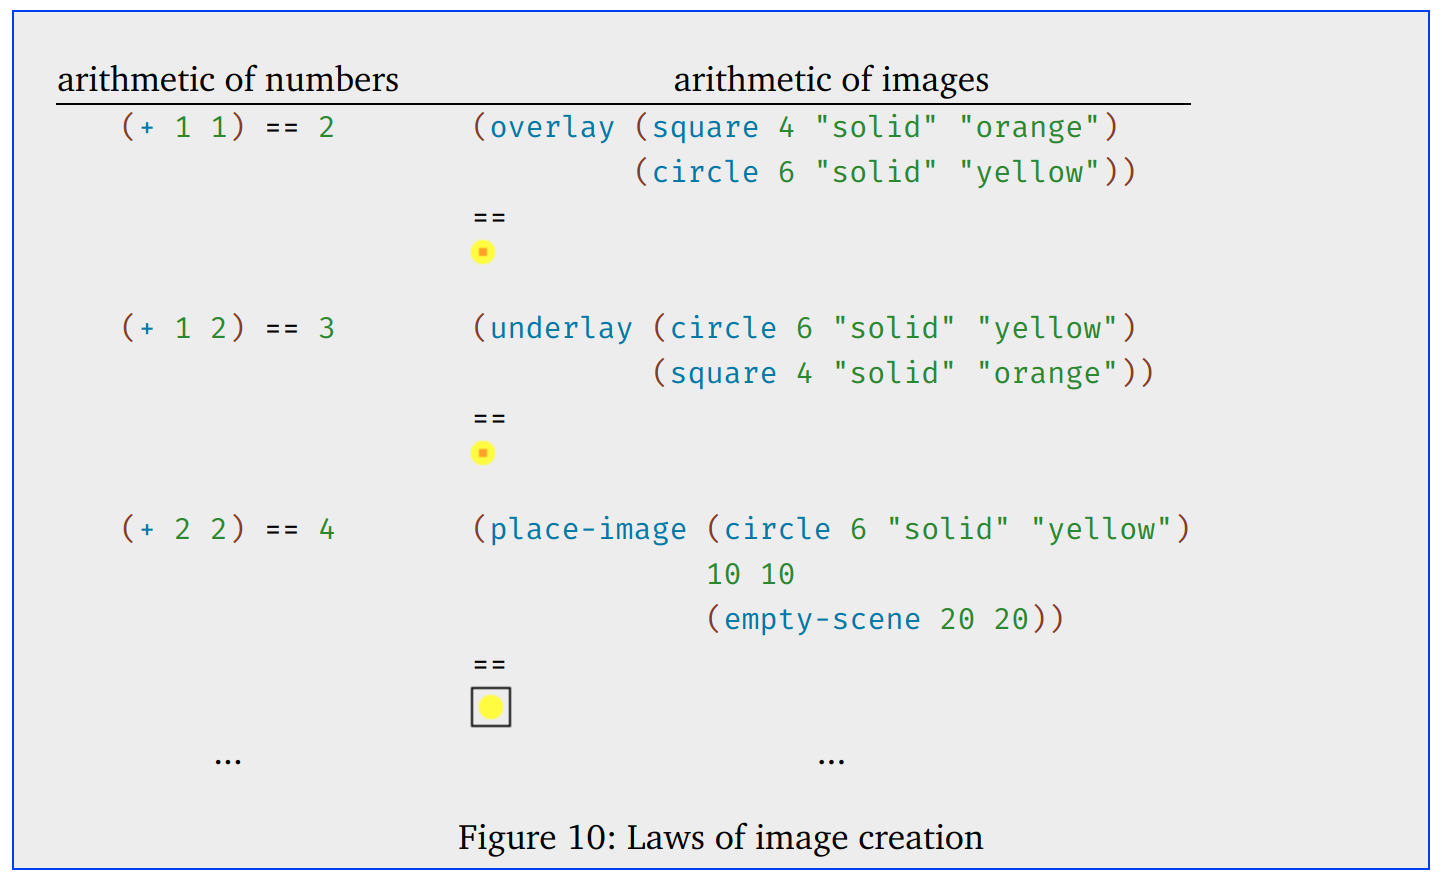
\includegraphics[width=0.7\textwidth]{images/Arithmetic-Images.png}
  \end{center}
\end{frame}

% \defverbatim[colored]\schemeTrue{
% \begin{minted}{Scheme}
%   #t
% \end{minted}
% }

\defverbatim[colored]\cond{
\begin{minted}{Scheme}
    (cond 
      [(> x 0) 1]
      [(= x 0) 0]
      [else -1])
\end{minted}
}

\begin{frame}
  \frametitle{Arithmetic of Booleans}
  Boolean Arithmetic should look familiar to all of you.
  \begin{itemize}
  \item<2-> The primitive boolean values are: 
    \text{\#t} and \text{\#f}
  \item<3-> The functions \mintinline{Scheme}{and}, \mintinline{Scheme}{or}, and
    \mintinline{Scheme}{not} do exactly what you expect
  \item<4-> We can write conditional expressions with the form:
    \mintinline{Scheme}{(if test-exp true-branch else-branch)}
  \item<5-> What does the following expression evaluate to?
    \mintinline{Scheme}{(+ 1 (if (< 0 1) 1 2))}
  \item<6-> When we have more conditions we use \mintinline{Scheme}{cond}:
    \cond
  \end{itemize}  
\end{frame}

\defverbatim[colored]\catProgram{
\begin{minted}{Scheme}
    (define cat-height (image-height cat))
    (define cat-width (image-width cat))
    
    (if (>= cat-height cat-width) 
        "long cat!" 
        "heckin chonker!")
\end{minted}
}

\begin{frame}
  \frametitle{Our First Program}
  Let's write a program to classify whether this cat is a long cat or a heckin
  chonker!
  \begin{center}
    
\includegraphics[width=0.1\textwidth]{images/cat.png}    
  \end{center}
  \begin{itemize}
  \item<2-> It should be a long cat if its height (tail height counts) is higher
    than its width.
  \item<3-> Help me write it! We're going to need
    \mintinline{Scheme}{image-height} and \mintinline{Scheme}{image-width}.
  \item<4-> Here it is: \catProgram
  \end{itemize}
\end{frame}

\begin{frame}
  \frametitle{Predicates}
  Predicates are a short way of saying boolean valued function. Let's take
  a look at some important predicates in Racket.
  \begin{itemize}
  \item<2-> We can check if something is a number with \mintinline{Scheme}{number?}
  \item<3-> \mintinline{Scheme}{(number? 2)}, \mintinline{Scheme}{(number? 2.3)}, and \mintinline{Scheme}{(number? 2/3)} all return true
  \item<4-> Surprisingly \mintinline{Scheme}{(rational? 2)}, \mintinline{Scheme}{(rational? (sqrt 2))}, and \mintinline{Scheme}{(rational? 2/3)} all return true too. 
  \item<5-> Use \mintinline{Scheme}{(exact? (sqrt 2))} or \mintinline{Scheme}{(inexact? (sqrt 2))}
  \item<6-> There are many other predicates: \mintinline{Scheme}{real?},
    \mintinline{Scheme}{boolean?}, \mintinline{Scheme}{image?},
    \mintinline{Scheme}{string?}, \mintinline{Scheme}{complex?}, ...
  \end{itemize}
\end{frame}

\defverbatim[colored]\predicateSkeleton{
\begin{minted}{Scheme}
    (cond
      [(... in) ...]
      ...)
\end{minted}
}

\defverbatim[colored]\predicatePartial{
\begin{minted}{Scheme}
    (cond
      [(string? in) ...]
      ...)
\end{minted}
}
\defverbatim[colored]\predicateFinal{
\begin{minted}[fontsize=\footnotesize]{Scheme}
    (cond 
        [(string? in) (string-length in)]
    	[(and (number? in) (> in 0)) (sub1 in)]
    	[(image? in) (* (image-height in) (image-width in))]
    	[else in])
\end{minted}
}
\begin{frame}
  \frametitle{Programming With Predicates}
  Create an expression that converts the value of \mintinline{Scheme}{in} to a positive number. For a String, it determines how long the String is; for an Image, it uses the area; for a Number, it decrements the number by 1, unless it is already 0 or negative; for true it uses 10 and for false 20.
\begin{itemize}
\item<2-> Let's diagram this out.
\item<3-> Here is our skeleton: \predicateSkeleton
%\item<4-> \predicatePartial
\item<4-> Here is our final version: \predicateFinal
\end{itemize}

\end{frame}

% \begin{frame}
%   \frametitle{Booleans and Conditionals}
%   \begin{itemize}
%   \item<2-> The structure of basic conditional statements:
%     \mintinline{Scheme}{(if test-exp true-branch else-branch)}
%   \item<3-> \mintinline{Scheme}{(if #t 1 2) ;;produces 1}
%   \item<4-> Can use it as an argument to other operations:
%     \mintinline{Scheme}{(+ 1 (if #t 1 2))}
%   \item<5-> This means that conditionals in Racket are expressions.
%   \item<6-> If we don't want to nest if-expressions, we use \mintinline{Scheme}{cond}
%   \item<7-> \mintinline{Scheme}{(cond [test-1 result-1] ...[test-n result-n])}
%   \item<8-> Let's record the sign of some integer x: \cond
%   \end{itemize}
% \end{frame}


\section{From Arithmetic to Functions}
\begin{frame}
  \frametitle{Our Bread and Butter}
  \begin{center}
    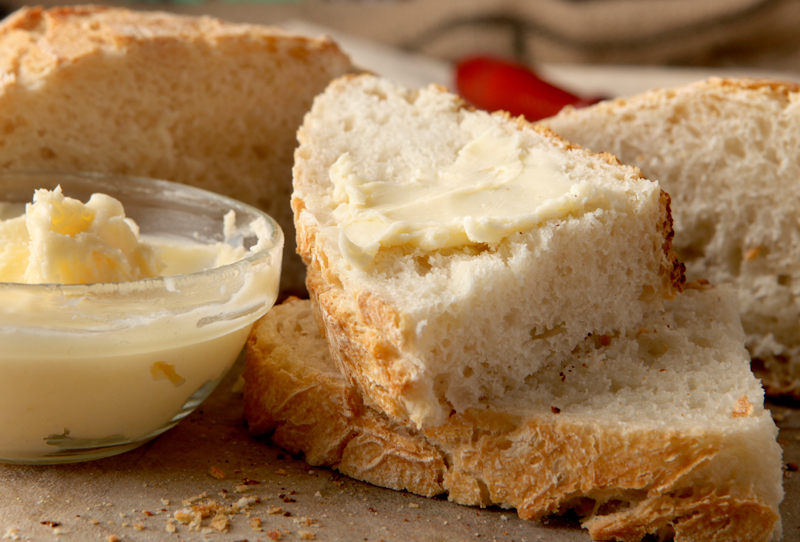
\includegraphics[width=0.4\textwidth]{images/bread-butter.jpg}
  \end{center}
  \begin{itemize}
  \item<2-> Yum!
  \item<3-> Functions are the bread and butter of functional programming, so let's get that bread!
  \item<4-> \huge But first, what is a function?
  \end{itemize}
\end{frame}



\begin{frame}
  \frametitle{The Algebra of Programming}
  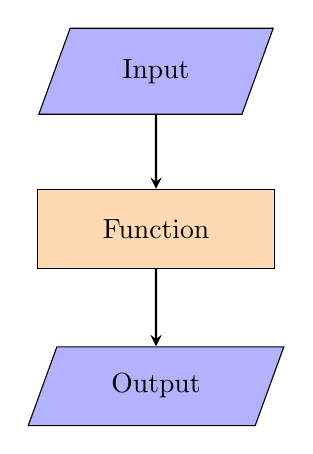
\begin{tikzpicture}[node distance=2cm]
    %\node (start) [startstop] {Start};
    \node (in1) [io] {Input};
    \node (pro1) [process, below of=in1] {Function};
    \node (out1) [io, below of=pro1] {Output};
    \draw [arrow] (in1) -- (pro1);
    \draw [arrow] (pro1) -- (out1);
  \end{tikzpicture}  
\end{frame}
\end{document}

